\section{Main Window}
\label{sec:ui_main_window} 

When the application is started for the first time, the main window is shown as follows. 

\begin{figure}[H]
  \hspace*{-2.5cm}
    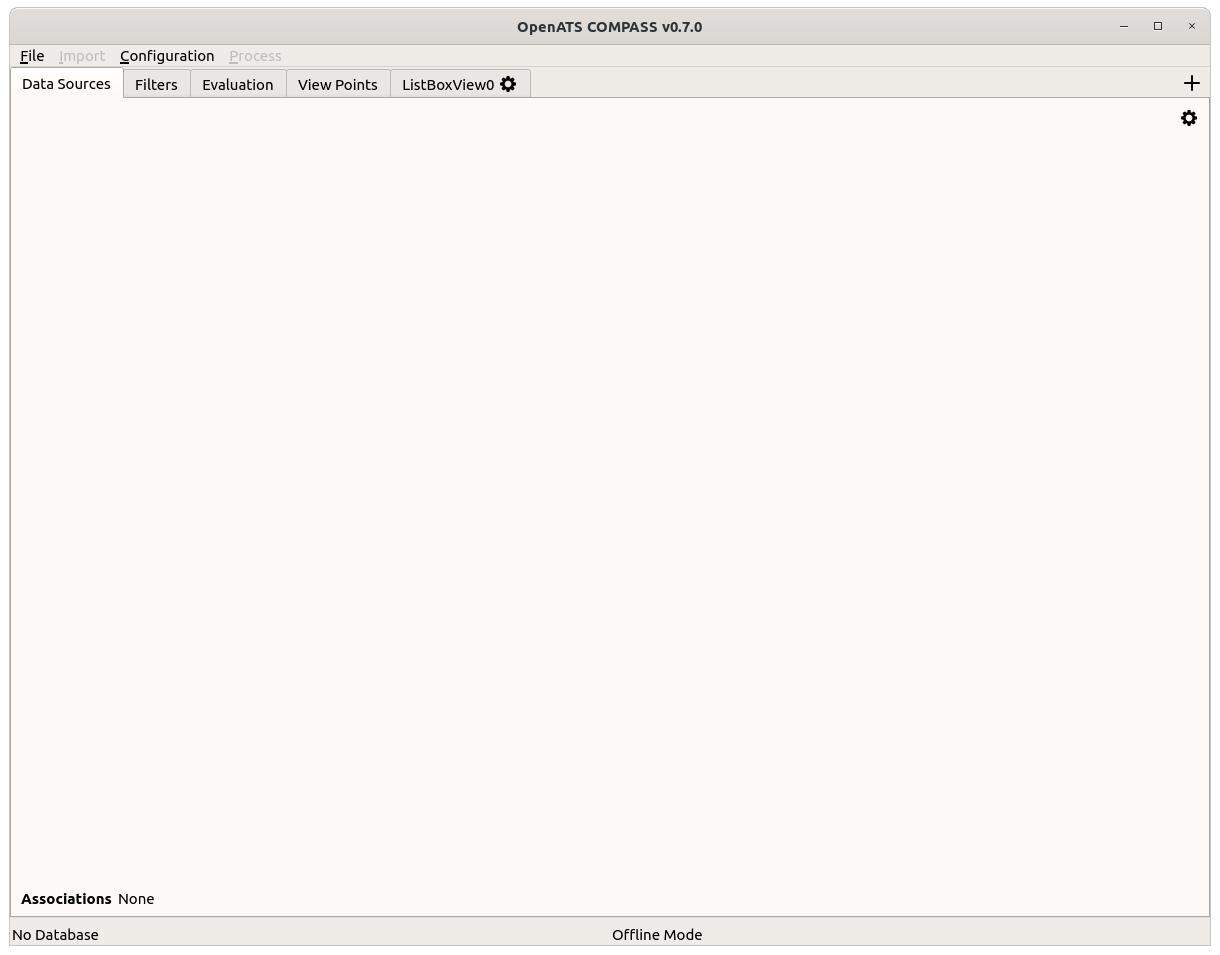
\includegraphics[width=19cm]{figures/main_window.png}
  \caption{Main Window}
\end{figure}

TODO short usage story, access db, add / process data, load/display data, close app \\
TODO links \\

\subsection{Main Menubar}

TODO story db -> worflow until loading/display data \\

At the top exists a main menubar, which allows access to the following groups:

\begin{itemize}
 \item File: Open/close a database, quit application
 \item Import: Import ASTERIX, NMEA data
 \item Configuration: Configure data sources, sectors
 \item Process: Various processing tasks for imported data
\end{itemize}
\  \\

\subsection{Main Tab Area}

TODO story what data is loaded into what views. views in other windows. add views \\

In the center, a number of tabs exist:
\begin{itemize}
 \item Data Sources: Select which data sources should be loaded
 \item Filter: Filter which data should be loaded
 \item Evaluation: Evaluate data according to given requirements
 \item View Points: Show/edit specific cases saved as View Points
 \item Views: All views included in the main window, e.g. ListBoxView0
\end{itemize}
\  \\

\subsection{Main Statusbar}

TODO shows status/mode, allows loading. views also load buttons \\

In the bottom, the following is shown:

In the center, a number of tabs exist:
\begin{itemize}
 \item Database indicator: Shows 'No Database' or currently opened database file
 \item Application mode: Offline or Live
 \item 'Load' button: Only visible when database was opened
\end{itemize}
\  \\

\subsection{Other Windows}

TODO add views, close other window deletes views, not close app \\

Depending on the status, some parts of the UI are inaccessible, e.g. are only available depending whether a database was opened.

